\documentclass[12pt]{article}
% Full article preamble (duplicated, no common file)
\usepackage{fontspec}
\usepackage[a4paper,margin=2.5cm,includefoot]{geometry}
\usepackage{polyglossia}
\usepackage{amsmath}
\usepackage{amssymb}
\usepackage{xcolor}
\usepackage{fancyhdr}
\usepackage{graphicx}
\usepackage{listings}
\usepackage[most]{tcolorbox}
\usepackage{pifont}
\usepackage{enumitem}
\usepackage{titlesec}
\usepackage[bottom]{footmisc}
\usepackage{titling}
\usepackage{minted}
\usepackage{etoolbox}
\usepackage{array}
\usepackage{extsizes}

\newfontfamily\emoji{Segoe UI Emoji}

\pagestyle{fancy}

\setmainlanguage[numerals=western]{arabic}
\setotherlanguage{english}
\newfontfamily\arabicfont[Script=Arabic]{Amiri}
\newfontfamily\arabicfonttt[Script=Arabic]{Courier New}

\lstset{
  language=[Sharp]C,
  numbers=left,
  stepnumber=1,
  numbersep=8pt,
  frame=single,
  basicstyle=\ttfamily\small,
  keywordstyle=\color{blue},
  stringstyle=\color{red},
  commentstyle=\color{green!50!black}
}

\newif\ifdetailed
\ifdefined\setdetailed
  \setdetailed
\fi

\newif\ifwithsols
\ifdefined\setwithsols
  \setwithsols
\fi

% unified tcolorboxes for articles
\tcbset{colback=white, colframe=black, fonttitle=\bfseries, boxrule=0.8pt}
\newtcolorbox{boxDef}[1][]{colback=blue!5!white,colframe=blue!75!black,
  title={{\emoji📘} تعريف\ifx\\#1\\\else ~#1\fi :}}
\newtcolorbox{boxExercise}[1][]{colback=cyan!5!white,colframe=cyan!70!black,
  title={{\emoji🧩} تمرين\ifx\\#1\\\else ~#1\fi :}}
\newtcolorbox{boxExample}[1][]{colback=yellow!5!white,colframe=orange!90!black,
  title={{\emoji📝} مثال\ifx\\#1\\\else ~#1\fi :}}
\newtcolorbox{boxNote}[1][]{colback=gray!10!white,colframe=black,
  title={{\emoji✨} ملاحظة\ifx\\#1\\\else ~#1\fi :}}
\newtcolorbox{boxAttention}[1][]{colback=magenta!10!white,colframe=magenta!80!black,
  title={{\emoji🔔} تنبيه\ifx\\#1\\\else ~#1\fi :}}
\newtcolorbox{boxWarning}[1][]{colback=red!5!white,colframe=red!75!black,
  title={{\emoji⚡} ملاحظة هامة\ifx\\#1\\\else ~#1\fi :}}
\newtcolorbox{boxSolution}[1][]{colback=green!5!white,colframe=green!60!black,
  title={{\emoji✅} حل\ifx\\#1\\\else ~#1\fi :}}
\newtcolorbox{boxSymbol}[1][]{colback=purple!5!white,colframe=purple!70!black,
  title={{\emoji🔣} رمز\ifx\\#1\\\else ~#1\fi :}}

\tcbset{simplecode/.style={ colback=gray!5, colframe=black!50, boxrule=0.4pt, arc=2pt, left=4pt,right=4pt,top=4pt,bottom=4pt}}
\newenvironment{boxCode}{\begin{tcolorbox}[simplecode]}{\end{tcolorbox}}

\newcolumntype{C}[1]{>{\centering\arraybackslash}p{#1}}

% redefine spaces after titles
\makeatletter
\renewcommand{\@maketitle}{%
  \begin{center}
    {\huge \bfseries \@title \par}%
    \vskip 0.2em % space between title and author
    {\large \@author \par}%
    % \vskip 0.2em % space between author and date
    % {\normalsize \@date \par}%
  \end{center}
}
\makeatother

\fancyhf{} % clear default
\fancypagestyle{plain}{
  \fancyhf{}
  \fancyhead[L]{مدرسة التسامح الشاملة}
  % \fancyhead[L]{
\includegraphics[height=1cm]{../../../images/logoTasamoh.png}}
  \fancyhead[R]{الأستاذ محمود اغبارية}
  \fancyfoot[C]{\thepage}
}

\fancyhead[L]{مدرسة التسامح الشاملة}
\fancyhead[R]{الأستاذ محمود اغبارية}
\fancyfoot[C]{\thepage}
% \date{\today}

\setcounter{tocdepth}{3} % only section subsection and subsubsection in TOC


% ----------------------


% \begin{document}

% \maketitle

% % \clearpage  % start TOC on a new page
% % \renewcommand{\contentsname}{جدول المحتويات}
% % \tableofcontents
% % \clearpage

% \part*{part 1} % the * prevents numbering
% \section*{مقدمة}
% \subsection*{مثال رياضي}
% \subsubsection*{مثال فرعي}
% \paragraph*{ paragraph 1}
% \subparagraph*{sub paragraph 1}

% \ifdetailed
% \begin{english}
% \begin{minted}{csharp}
% // C# Example
% \end{minted}
% \end{english}
% \fi

% OLD WAY
% \ifdetailed
% \begin{english}
% \begin{lstlisting}
% // C# Example
% \end{lstlisting}
% \end{english}
% \fi

% % 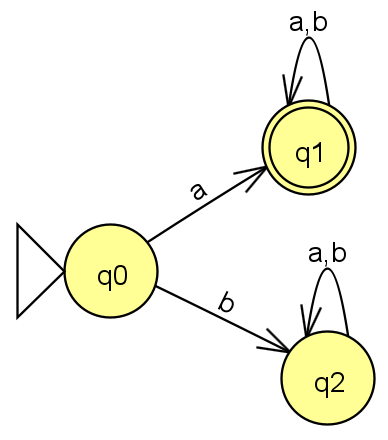
\includegraphics[width=0.2\textwidth]{../../../images/DFAs/ex1_q1.png}



% \vspace{3cm}
% \begin{flushleft}
% أرجو لكم وقتًا ممتعًا.

% الأستاذ محمود اغبارية.
% \end{flushleft}


% \end{document}


\title{تمرين 1 للصف 11-10 - اوتومات نهائي محدّد}

\begin{document}

\maketitle

\section{تحديد لغة الأوتومات}

حدد لغة كل أوتومات من التالية:

\ifwithsols
\begin{enumerate}[itemsep=3em]
\else
\begin{enumerate}
\fi

\item
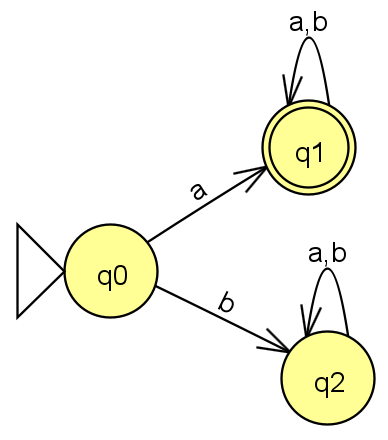
\includegraphics[width=0.3\textwidth]{../../../images/DFAs/ex1_q1.png}\\
\ifwithsols
\begin{solution}
\[ L = a \cdot \{a,b\}^* \]
لغة كل الكلمات التي تبدأ بالحرف $a$.
\end{solution}
\fi

\item
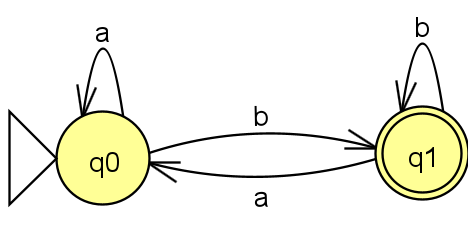
\includegraphics[width=0.3\textwidth]{../../../images/DFAs/ex1_q2.png}\\
\ifwithsols
\begin{solution}
    \[ L = \{a,b\}^* \cdot b \]
    لغة كل الكلمات التي تنتهي بالحرف $b$.
\end{solution}
\clearpage
\fi

\item
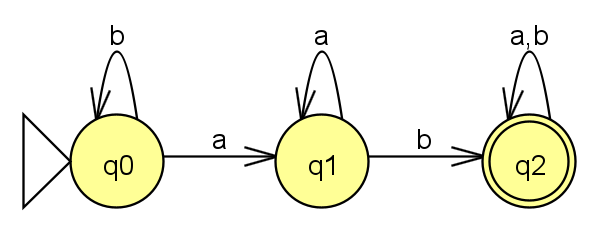
\includegraphics[width=0.4\textwidth]{../../../images/DFAs/ex1_q3.png}\\
\ifwithsols
\begin{solution}
\[ L = b^* \cdot a \cdot a^* \cdot b \cdot \{a, b \}^* = b^* \cdot a^+ \cdot b \cdot \{a,b\}^* \]
لغة كل الكلمات التي تحتوي على الحرف $a$ ثم يظهر على الأقل $b$ واحد بعده.
\end{solution}
\fi

\item
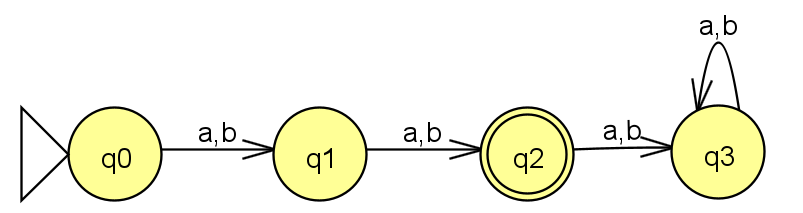
\includegraphics[width=0.5\textwidth]{../../../images/DFAs/ex1_q4.png}\\
\ifwithsols
\begin{solution}
\[ L = \{a, b\}^2 = \{ w \in \{a,b\}^* \mid |w|=2 \} \]
كل الكلمات التي طولها بالضبط 2.
\end{solution}
\fi

\item
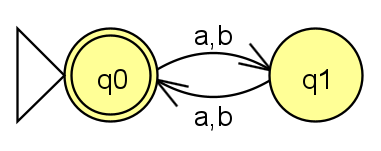
\includegraphics[width=0.25\textwidth]{../../../images/DFAs/ex1_q5.png}\\
\ifwithsols
\begin{solution}
\[ L = \{ w \in \{a,b\}^* \mid |w| \% 2 = 0 \} \]
كل الكلمات التي طولها زوجي. \\
\textbf{انتبه}: $\epsilon \in L$ لأنّ $|\epsilon|=0$ وهو زوجي، وهذا يناسب الأوتومات حيث إنّ $q_0$ حالة قابلة.
\end{solution}
\fi

\item
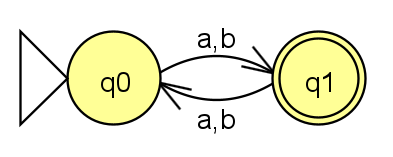
\includegraphics[width=0.25\textwidth]{../../../images/DFAs/ex1_q6.png}\\
\ifwithsols
\begin{solution}
\[ L = \{ w \in \{a,b\}^* \mid |w| \% 2 = 1 \} \]
كل الكلمات التي طولها فردي.
\end{solution}
\fi

\item
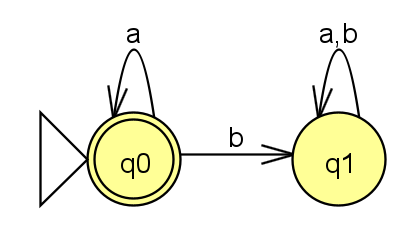
\includegraphics[width=0.3\textwidth]{../../../images/DFAs/ex1_q7.png}\\
\ifwithsols
\begin{solution}
\[ L = a^* \]
كل الكلمات التي لا تحتوي على $b$. \\
\textbf{انتبه}: $\epsilon \in L$ لأنّ $\epsilon = a^0$ لا يحتوي على $b$، وهذا يناسب الأوتومات حيث إنّ $q_0$ حالة قابلة.
\end{solution}
\fi

\item
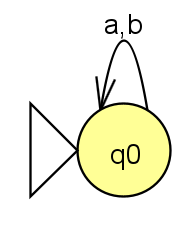
\includegraphics[width=0.1\textwidth]{../../../images/DFAs/ex1_q8.png}\\
\ifwithsols
\begin{solution}
\[ L = \emptyset \]
هذا الأوتومات لا يقبل أي كلمة.
\end{solution}
\fi

\item
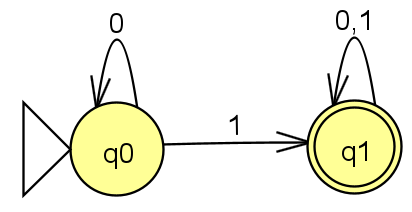
\includegraphics[width=0.3\textwidth]{../../../images/DFAs/ex1_q9.png}\\
\ifwithsols
\begin{solution}
\[ L = 0^* \cdot 1 \cdot \{0, 1\}^* \]
كل الكلمات التي تحتوي على $1$ على الأقل.
\end{solution}
\fi

\item
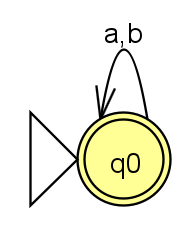
\includegraphics[width=0.1\textwidth]{../../../images/DFAs/ex1_q10.png}
\ifwithsols
\begin{solution}
\[ L = \{a, b\}^* \]
هذا الأوتومات يقبل كل الكلمات.
\end{solution}
\fi

\item
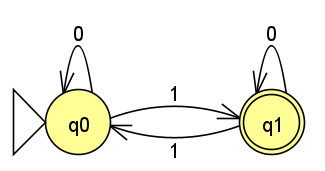
\includegraphics[width=0.3\textwidth]{../../../images/DFAs/ex1_q11.png}
\ifwithsols
\begin{solution}
\[ L = \{ w \in \{0, 1\}^* \mid \#_1(w) \% 2 = 1 \} \]
كل الكلمات التي يظهر فيها الحرف $1$ عدد مرات فردي.
\end{solution}
\fi

\item
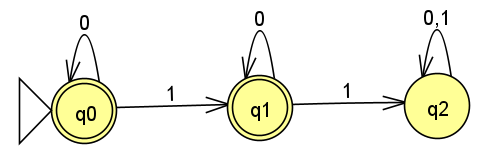
\includegraphics[width=0.4\textwidth]{../../../images/DFAs/ex1_q12.png}
\ifwithsols
\begin{solution}
\[ L = \{ w \in \{0, 1\}^* \mid \#_1(w) \leq 1 \} \]
كل الكلمات التي يظهر فيها الحرف $1$ مرة واحدة على الأكثر. \\
\textbf{انتبه}: $\epsilon \in L$ لأنّ $\epsilon$ لا يحتوي على $1$، وهذا يناسب الأوتومات حيث إنّ $q_0$ حالة قابلة.
\end{solution}
\fi

\item
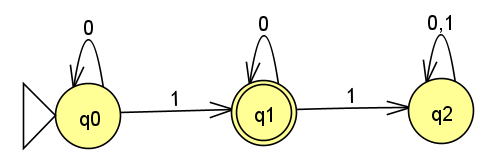
\includegraphics[width=0.4\textwidth]{../../../images/DFAs/ex1_q13.png}
\ifwithsols
\begin{solution}
\[ L = \{ w \in \{0, 1\}^* \mid \#_1(w) = 1 \} \]
كل الكلمات التي يظهر فيها الحرف $1$ مرة واحدة بالضبط.
\end{solution}
\fi

\end{enumerate}

\clearpage
\section{أكمل الناقص في الأتومات}
أكمل الناقص في الأوتوماتات التالية بحيث تقبل اللغة الموضحة.

\ifwithsols
\begin{enumerate}[itemsep=3em]
\else
\begin{enumerate}
\fi

\item
\textbf{اللغة:} كل السلاسل من الأبجدية $\{a, b, c\}$ التي فيها (عدد الـ $a$ + عدد الـ $b$) هو عدد فردي.
\[ L = \left\{ w \in \{a, b, c\} \mid (\#_a(w) + \#_b(w)) \% 2 = 1 \right\} \]
\begin{center}
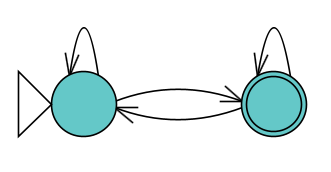
\includegraphics[width=0.4\textwidth]{../../../images/DFAs/ex1_p2_q1.png}
\end{center}
\ifwithsols
\begin{solution}
    \begin{center}
        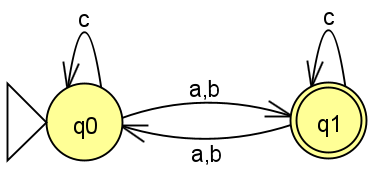
\includegraphics[width=0.4\textwidth]{../../../images/DFAs/ex1_p2_q1_sol.png}
    \end{center}
\end{solution}
\fi

\item
\textbf{اللغة:} كل السلاسل من الأبجدية $\{0, 1, 2\}$ التي مجموع الخانات فيها هو عدد فردي.
\begin{center}
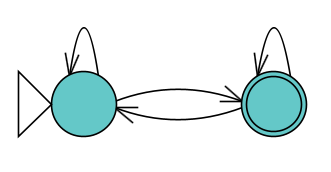
\includegraphics[width=0.4\textwidth]{../../../images/DFAs/ex1_p2_q1.png}
\end{center}
\ifwithsols
\begin{solution}
    \begin{center}
        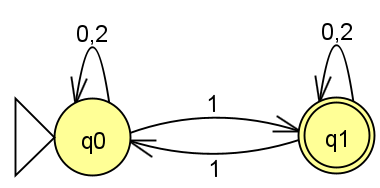
\includegraphics[width=0.4\textwidth]{../../../images/DFAs/ex1_p2_q2_sol.png}
    \end{center}
\end{solution}
\clearpage
\fi

\item
\textbf{اللغة:} كل السلاسل من الأبجدية $\{a, b\}$ التي تبدأ بالحرف $a$ وتنتهي بالحرف $b$.
\[ L = a \cdot \{a, b\}^* \cdot b \]
\begin{center}
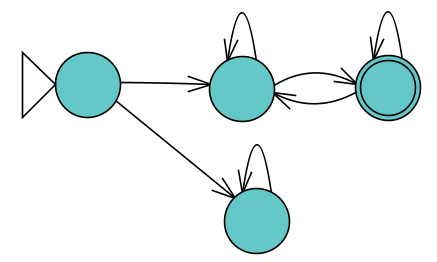
\includegraphics[width=0.5\textwidth]{../../../images/DFAs/ex1_p2_q3.png}
\end{center}
\ifwithsols
\begin{solution}
    \begin{center}
        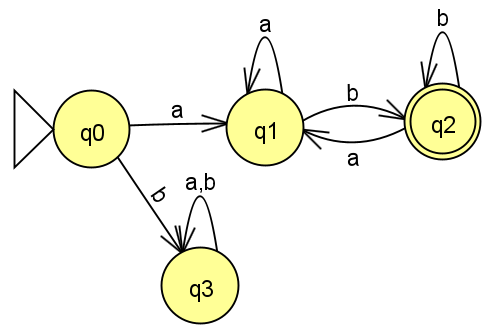
\includegraphics[width=0.4\textwidth]{../../../images/DFAs/ex1_p2_q3_sol.png}
    \end{center}
\end{solution}
\fi

\end{enumerate}


\clearpage
\section{بناء أوتومات من اللغة}

لكل لغة من اللغات التالية، ابنِ أوتوماتًا يقبل هذه اللغة، واكتب تعبيرًا رياضيًّا يصف اللغة.

\begin{enumerate}

\item
\textbf{اللغة:} كل السلاسل من الأبجدية $\{0, 1\}$ التي تحتوي على $1$ واحدة على الأقل.

\item
\textbf{اللغة:} كل السلاسل من الأبجدية $\{0, 1\}$ التي لها عدد زوجي من الأصفار.

\item
\textbf{اللغة:} كل السلاسل من الأبجدية $\{0, 1\}$ حيث كل $0$ تتبعها مباشرة $1$.

\item
\textbf{اللغة:} كل السلاسل من الأبجدية $\{a, b\}$ التي تبدأ وتنتهي بنفس الحرف.

\item
\textbf{اللغة:} كل السلاسل من الأبجدية $\{0, 1\}$ التي طولها يقبل القسمة على 3.

\item
\textbf{اللغة:} كل السلاسل من الأبجدية $\{a, b, c\}$ التي لا تحتوي على السلسلة الفرعية $ac$.

\item
\textbf{اللغة:} كل السلاسل من الأبجدية $\{a, b\}$ التي لها عدد فردي من الحرف $a$ وعدد فردي من الحرف $b$.

\item
\textbf{اللغة:} كل السلاسل من الأبجدية $\{a, b\}$ التي تحتوي على عدد زوجي من $a$ أو عدد زوجي من $b$.

\item
\textbf{اللغة:} اللغة التي تحتوي على السلسلة $baba$ فقط.

\item
\textbf{اللغة:} كل السلاسل من الأبجدية $\{a, b\}$ التي لا تنتهي بـ $ab$.

\item
\textbf{اللغة:} كل السلاسل من الأبجدية $\{a, b\}$ التي من الصورة $m,n>0, \{a^mb^n\}$

\item
\textbf{اللغة:} كل السلاسل من الأبجدية $\{a, b\}$ التي تحتوي على السلسلة الفرعية $aba$.

\item
\textbf{اللغة:} كل السلاسل من الأبجدية $\{a, b\}$ التي فيها عدد الـ $a$ يقبل القسمة على 3.

\item
\textbf{اللغة:} كل السلاسل من الأبجدية $\{a, b\}$ التي لا تحتوي على $aa$ (أي لا يوجد حرفان $a$ متتاليان).

\item
\textbf{اللغة:} كل السلاسل من الأبجدية $\{a, b\}$ التي هي من الصورة $(ab)^n$ حيث $n \ge 1$. \\
(مثل: $ab, abab, ababab, \dots$)

\item
\textbf{اللغة:} كل السلاسل من الأبجدية $\{a, b\}$ ذات الطول الزوجي والتي تنتهي بالحرف $a$.

\item
\textbf{اللغة:} كل السلاسل من الأبجدية $\{0, 1\}$ التي لها عدد زوجي من $0$ وعدد فردي من $1$.

\item
\textbf{اللغة:} كل السلاسل من الأبجدية $\{0, 1, 2\}$ التي مجموع خاناتها يقبل القسمة على 3.

\item
\textbf{اللغة:} كل السلاسل من الأبجدية $\{a, b\}$ التي تحتوي على حرف $b$ مرّتين على الأقل (ليس بالضرورة متتاليتين).

\item
\textbf{اللغة:} كل السلاسل من الأبجدية $\{a, b\}$ التي تبدأ بـ $a$ ولا تحتوي على السلسلة الفرعية $bb$.

\end{enumerate}

\end{document}
